% \begin{question}{Warum kommt es zu Riesenresonanzen oder Plasmonen? Eine Spinwelle oder ein Phonon sind doch auch eine kollektive Anregung, trotzdem gibt es hier keinen Sprung in den Energieskalen?}
%     Resonanz ist das Stichwort, 'peaks' jeglicher Art sind dafür typisch
%     Phononen und Spinwellen sind wie Photonen, bei denen gibt es ja auch nicht grundsätzlich einen Sprung in der Anregungsenergie, außer eben bei Plasmonen
% \end{question}

\begin{fquestion}{Was sind die relevanten Größenordnungen bei Dipolriesenresonanzen (GDR) und Oberflächenplasmonen (SPR)?}
   GDR: $E\approx (7\dots 40)\,$MeV, beruht auf starker Wechselwirkung (Kernkraft, Oberflächenterme), Anregung durch Photonen und Neutronen %(auch durch Elektronen mit $E\gtrsim 50\,$MeV über eine Art umgekehrter innerer Konversion ??? )
   \\
   SPR: $E\sim 1\,$eV (optisches Spektrum, $\omega \simeq \omega_\mathrm{plasma}$ !), beruht auf elektromagnetischer Wechselwirkung (Coulomb, Polarisation), Anregung durch Photonen
\end{fquestion}

\subsection{Plasmonen}

\begin{fquestion}{Was sind Plasmonen?}
    Plasmonen sind quantisierte Schwingungen der Elektronendichte. 
    Sie sind somit eine kollektive Schwingungsanregung von Elektronen. 
    Die Dispersionsrelation von Oberflächenplasmonen
    \[\omega = \omega_p \sqrt{1 + \frac{c^2k^2}{\varepsilon(\infty)}}.\]
    
    \begin{center}
        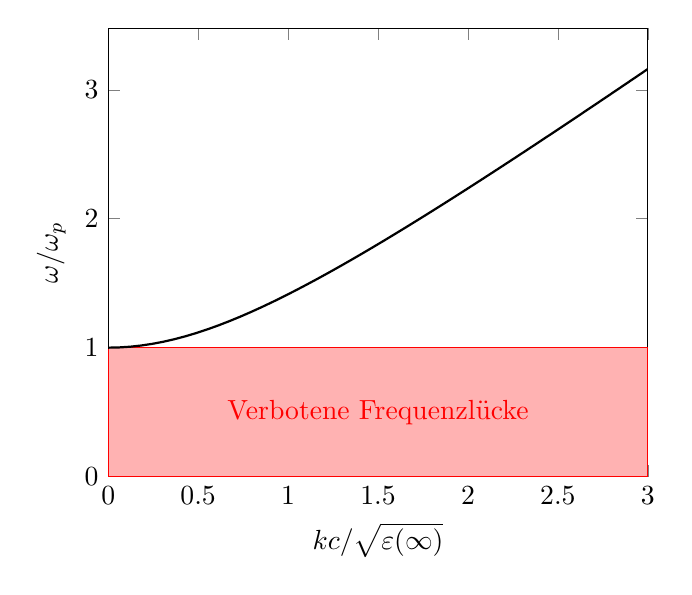
\begin{tikzpicture}
            \centering
            \begin{axis}[domain=0:3, xmin=0, xmax=3, ymin=0, xlabel = {$k c / \sqrt{\varepsilon(\infty)}$}, ylabel = {$\omega / \omega_p$}]
                \draw[red, fill = red!30!white] (0,0) rectangle (3,1) node[pos=.5] {Verbotene Frequenzlücke};
                \addplot [thick, black, samples=50] {sqrt(1 + x^2)};
            \end{axis}
        \end{tikzpicture}
    \end{center}
\end{fquestion}

% \begin{fquestion}{Wodurch werden Plasmonen angeregt?}
%     Photonen
% \end{fquestion}

\begin{fquestion}{Warum nutzt man zur Anregung von Plasmonen keine Neutronen?}
    Neutronen besitzen keine äußere Ladung und können daher nur über das magnetische Moment wechselwirken.
    Diese Anregung ist schwächer als die elektromagnetische Anregung über Photonen.
\end{fquestion}

\begin{fquestion}{Von was hängt die Plasmafrequenz ab?}
    Sie ist abhängig von der Elektronendichte $n_e$ und der effektiven Masse $m^\star$ der Elektronen 
    \[\omega_p = \sqrt{\frac{n_e e^2}{m^\star \varepsilon_0}}\]
\end{fquestion}

\begin{fquestion}{Wie ist der Zusammenhang zwischen Plasmonen und den optischen Eigenschaften von Metallen?}
    Unterhalb der Plasmafrequenz können Plasmonen durch die Interaktion mit den Photonen erzeugt werden, diese werden also absorbiert (und durch Rückkopplung der Plasmonen mit der Luft entsprechend reflektiert).
    Oberhalb der Plasmafrequenz geschieht dies nicht und die Photonen werden transmittiert.
    
    Da die Plasmafrequenz bei den meisten Metallen im ultravioletten liegt, erhalten sie ihren typischen metallischen Glanz.
\end{fquestion}

% \begin{question}{Was schwingt im Zusammenhang mit Reflexion?}
%     Licht mit einer Frequenz über der Plasmafrequenz ist transmittiert, Licht mit einer Frequenz unter der Plasmafrequenz ist relfektiert. 
%     bei höherer Frequenz können die Elektronen nicht schnell genug reagieren??? (Erklärung Wikipedia, komisch)
% \end{question}

\begin{fquestion}{Wo treten Plasmonen auf?}
    In Metallen und Halbleitern. 
    In Halbleitern kann man über Dotierung die Elektronendichte steuern und somit die Plasmafrequenz und die Reflektivität einstellen.
\end{fquestion}

\subsection{Riesenresonanzen}

% \begin{question}{Durch welches Potential werden Atomkerne im Schalenmodell beschrieben?}
%     Durch das Woods-Saxon-Potential
%     \[V(r) = \frac{-V_0}{1 + \exp\left(\frac{r - R}{a}\right)}\]
%     mit Potentialtiefe $V_0 \approx \SI{40}{MeV}$, Radiusparameter $r_0 \approx \SI{1.2}{\femto\metre}$, Potentialrand $a \approx \SI{0.5}{\femto\metre}$ und Radius $R =  r_0 A^{1/3}$.
% \end{question}

\begin{fquestion}{Was sind Riesenresonanzen?}
    Riesenresonanzen sind kollektive Schwingungsanregungen von Nukleonen im Kern, invers zum $\gamma$-Zerfall. 
    Sie haben die Energien im Bereich von $10\ldots 40\, \si{\mega\electronvolt}$. 
    Sie haben hohe Energie und Wirkungsquerschnitt.  
    
    Abgeregt werden die Schwingungen durch Kernspaltung, $n$- oder $\alpha$-Emission.
\end{fquestion}

\begin{fquestion}{Was ist das Steinwedel-Jensen-Modell?}
    Das Steinwedel-Jensen-Modell erklärt Riesenresonanzen über Dichtebewegungen der Neutronen und Protonen als Fluid.
    Die Resonanz entspricht dann einer stehenden Welle mit Wellenlänge $\lambda \sim R$, wobei  $R$ der Kernradius ist.
    Insbesondere gilt dann $E_\mathrm{SJ} \sim \frac{1}{\lambda} \sim \frac{1}{A^{1/3}}$.
\end{fquestion}

\begin{fquestion}{Was ist das Goldhaber-Teller-Modell?}
    Im Goldhaber-Teller-Modell werden die Riesenresonanzen durch Schwingungen der Protonen gegen die Neutronenwolke beschrieben.
    Für die semiempirische Beschreibung ist der Oberflächenterm aus der Bethe-Weizsäcker-Formel interessant, da $E\sim \frac{(N_O - Z_O)^2}{A_O} \sim \frac{ (R^2)^2}{R^2} = R^2$ (der Index $O$ steht für die Nukleonen an der Oberfläche).
    Man kann die Schwingung dann als harmonischen Oszillator mit $E\sim R^2\Delta x^2 \overset{!}{\sim} m\omega^2\Delta x^2$ auffassen, woraus sich $E_\mathrm{GT}\sim \omega\sim \sqrt{\frac{R^2}{m}} \sim \sqrt{\frac{A^{2/3}}{A}} \sim \frac{1}{A^{1/6}}$ ergibt.
\end{fquestion}

\begin{fquestion}{Wie verändert sich die Riesenresonanz eines Isotops für verschiedene Massen?}
    Für einen kugelsymmetrischen Kern gibt es nur eine Schwingungsmode, die Resonanz beteht dann nur aus einem Peak.
    Durch Hinzufügen von Neutronen wird der Kern deformiert, wodurch es zwei unterschiedliche Moden gibt. 
    Das spiegelt sich dann in dem Aufspalten in zwei Peaks wieder (beispielsweise bei ${}^{142\dots 150}\mathrm{Nd}$).
\end{fquestion}

% \begin{question}{Wodurch werden Riesenresonanzen angeregt?}
%     Beispielsweise durch hochenergetische Neutronen, Photonen oder Elektronen. 
% \end{question}

\begin{fquestion}{Warum kann ${}^{235}\mathrm{U}$ durch Neutronen gespalten werden, ${}^{238}\mathrm{U}$ aber nicht?}
    Die Potentialbarriere bei großen Kernen ist ungefähr 6\,MeV. 
    Die Bindungsenergie der Neutronen bei ${}^{235}\mathrm{U}$ ist 6\,MeV und reicht als Aktivierungsenergie für die Kernspaltung. 
    Die Bindungsenergie der Neutronen bei ${}^{238}\mathrm{U}$ ist 4.8\,MeV und reicht nicht als Aktivierungsenergie, das Neutron müsste noch ca. 1\,MeV kinetische Energie haben.  
    
    Die Diskrepanz der Bindungsenergien kommt aus dem Paarungsterm, eine gerade Anzahl an Neutronen ist bevorzugt.
    Dabei hat ${}^{235}\mathrm{U}$ eine gerade Anzahl Neutronen, ${}^{238}\mathrm{U}$ nicht.
    
\end{fquestion}

\begin{fquestion}{Warum entstehen bei der Kernspaltung meistens ein leichter und ein schwerer Kern?}
    Kerne mit magischen Zahlen sind stabiler, ein asymmetrischer Zerfall ist daher energetisch günstiger, wenn die Tochterkerne nah an Kernen mit magischen Zahlen liegen. 
\end{fquestion}

\begin{fquestion}{Woher kommen die schweren Elemente im Universum?}
    Aus Supernovae und der Fusion von Neutronensternen.
    Dort werden bei der Fusion entstehende Elemente schnell mit Neutronen angereichert und können dann über $\beta^-$-Zerfall zu stabilen Elementen zerfallen.  
\end{fquestion}

\begin{fquestion}{Multipolstrahlung?}
    Die Paritätsänderung $\Delta P = \pm 1$ ist $\Delta P = (-1)^{\ell}$ für elektrische Übergänge $E_\ell$ und $\Delta P = -(-1)^{\ell}$ für magnetische Übergänge $M_\ell$.
    Hierbei steht $\ell = 1$ für Dipolstrahlung, $\ell = 2$ für Quadrupolstrahlung, etc.
    In der Tabelle sind diese für einige Werte aufgelistet.
    Der eingeklammerte Term entspricht jeweils der nächsthöheren Ordnung. 
    \begin{center}
    \begin{tabular}{c|c|c|c|c}
        $\Delta J$ & $0^\ast$ & 1 & 2 & 3 \\ \hline
        $\Delta P = -1$ & $E_1 (M_2)$ & $E_1 (M_2)$ & $M_2 (E_3)$ & $E_3 (M_4)$ \\
        $\Delta P = +1$ & $M_1 (E_2)$ & $M_1 (E_2)$ & $E_2 (M_3)$ & $M_3 (E_4)$ \\
    \end{tabular}
    \end{center}
    Für $\Delta J \in \{-1,0,+1\}$ gilt dann $\Delta L = \pm 1$ und $\Delta S = 0$ für elektrische Übergänge, und $\Delta L = 0$ und $\Delta S = \pm 1$ für magnetische Übergänge, damit jeweils die Paritätsänderung mit $\Delta L$ übereinstimmt.
    \\
    $0^\ast$: Der strahlungslose Übergang $0\rightarrow 0$ ist verboten.
\end{fquestion}

\begin{fquestion}{Ist der 1S Hyperfeinübergang in Wasserstoff über $E_1$-Dipolstrahlung möglich?}
    Nein, weil für einen $E_1$-Übergang $\Delta L = \pm 1$ gelten muss.
    Beim 1S-Übergang ist aber $\Delta L = 0$, womit zumindest der magnetische $M_1$-Übergang möglich ist.
    Dieser ist allerdings stark unterdrückt, da
    $$\Gamma_M \simeq \Gamma \left(\frac{p}{m_e}\right)^2 \approx \Gamma\alpha^2.$$
    Hierbei wurde $p\approx\frac{1}{r_0} = \alpha m_e$ verwendet.
    Der Faktor $\frac{p}{m_e}$ entspricht dabei näherungsweise $\frac{E_\gamma }{E_0}$ aus der theoretischen Vorhersage.
    Die klassische Abschätzung für die elektrische Dipolstrahlung ist $\Gamma = \frac{\alpha}{3} R^2E_\gamma^3 \approx \frac{E_\gamma^3}{3\alpha m_e^2}$ (mit $R\approx r_0$).
    Es gilt $E_\gamma \simeq \SI{6}{\micro eV}$, also
    $$\Gamma_M \approx \frac{\alpha E_\gamma^3}{3m_e^2} \approx \SI{2e-30}{eV}.$$
    Das entspricht einer Lebensdauer von $\tau_M = \frac{1}{\Gamma_M} \approx \SI{1e7}{a}$, was mit dem experimentellen Wert von $\SI{1.1e7}{a}$ gut übereinstimmt.
\end{fquestion}

\begin{fquestion}{In welchen Systemen kann man die elektrische Quadrupolstrahlung vernachlässigen?}
    Die Multipolentwicklung basiert auf $\e^{\i kr} \simeq 1 + \i kr + \frac{1}{2}(\i kr)^2 + \dots$, höhere Ordnungen sind also jeweils um einen Faktor $RE_\gamma$ unterdrückt.
    Für das Verhältnis von Quadrupolstrahlung ($E_2$) zu Dipolstrahlung ($E_1$) gilt dann $r := \frac{E_2}{E_1} \sim |RE_\gamma|^2$.
    \begin{center}
        \begin{tabular}{c|c|c|c}
             & $E_\gamma$ & $R$ & $r$ \\ \hline
            Atom & $\sim \SI{10}{eV}$ & $\sim \SI{0.1}{nm}$ & $\sim \frac{1}{40000}$ \\ 
            Kern & $\sim \SI{1}{MeV}$ & $\sim \SI{10}{fm}$ & $\sim \frac{1}{400}$ \\ 
            Meson & $\sim \SI{100}{MeV}$ & $\sim \SI{0.01}{MeV^{-1}}$ & $\sim 1$ \\ 
        \end{tabular}
    \end{center}
    Bei Mesonen wurde in der Tabelle die Abschätzung $R\sim \frac{1}{\alpha_s m_\mathrm{const}^\mathrm{quark}} \approx \frac{1}{0.1 \cdot \SI{1000}{MeV}}$ verwendet.
    Für Mesonen sind die höheren Momente also prinzipiell nicht vernachlässigbar.
\end{fquestion}    
% Man kann die Schwingung dann als harmonischen Oszillator mit $E\sim R^2\Delta x^2 \overset{!}{\sim} m\omega^2\Delta x^2$ auffassen, woraus sich $E_\mathrm{GT}\sim \omega\sim \sqrt{\frac{R^2}{m}} \sim \sqrt{\frac{A^{2/3}}{A}} \sim \frac{1}{A^{1/6}}$ ergibt.

